%
% File acl2018.tex
%
%% Based on the style files for ACL-2017, with some changes, which were, in turn,
%% Based on the style files for ACL-2015, with some improvements
%%  taken from the NAACL-2016 style
%% Based on the style files for ACL-2014, which were, in turn,
%% based on ACL-2013, ACL-2012, ACL-2011, ACL-2010, ACL-IJCNLP-2009,
%% EACL-2009, IJCNLP-2008...
%% Based on the style files for EACL 2006 by 
%%e.agirre@ehu.es or Sergi.Balari@uab.es
%% and that of ACL 08 by Joakim Nivre and Noah Smith

\documentclass[11pt,a4paper]{article}
\usepackage[hyperref]{acl2018}
\usepackage{times}
\usepackage{latexsym}
\usepackage{color}
\usepackage{url}
\usepackage{graphicx}
\graphicspath{{Figures/}}

\aclfinalcopy % Uncomment this line for the final submission
%\def\aclpaperid{***} %  Enter the acl Paper ID here

%\setlength\titlebox{5cm}
% You can expand the titlebox if you need extra space
% to show all the authors. Please do not make the titlebox
% smaller than 5cm (the original size); we will check this
% in the camera-ready version and ask you to change it back.

\newcommand\BibTeX{B{\sc ib}\TeX}

\title{Classifying Job Review Helpfulness Using Convolutional Neural Networks}

\author{Ryan Delgado \\
	datascience@berkeley.edu / W266: NLP with Deep Learning \\
	{\tt rmdelgad2013@berkeley.edu}
}

\date{}

\begin{document}
	\maketitle
	\begin{abstract}
		Employers and potential employees alike benefit from information about critical work environment elements like work-life balance or job satisfaction. They often turn to job review websites like Glassdoor obtain candid information about these company features. However, it is difficult to distinguish between which feedback is useful and which is not. This paper explores the collection and analysis of a novel dataset of job reviews scraped from company Glassdoor pages in order to attempt to classify reviews based on their ``Helpfulness". I compare using a baseline Support Vector Machine (SVM) with bigram word counts versus a Convolutional Neural Network (CNN) for this classification task. I experimented with different configurations of the CNN model, such as different dropout rates, filter sizes and numbers of filters, and using randomly-initialized or pre-trained embeddings. The CNN model underperformed the baseline model in this classification task, and the dropout rate had a significant impact on model performance, filter configurations did not impact performance, and using pre-trained embeddings boosted performance.
	\end{abstract}	
	
	\section{Introduction}
	Glassdoor (www.glassdoor.com) is a widely-used service that allows current and former employees to post anonymous ratings about their experience working at any company registered on the site. This allows potential employees to research companies before beginning employment, and provides employers the opportunity to obtain candid feedback about their work environment. Reviewers are asked to score companies overall on a five-star scale, and offered the opportunity to write about the positive and negative aspects of the company. Glassdoor has only a simple content approval process, so individuals seeking quality reviews may have to read through tens or even hundreds of reviews in order to gather enough information about a future employer. Glassdoor also provides a peer review system through the use of its ``Helpful" button, which allows review readers to rate any review they come across. However, no current standards exist to guide users regarding what Helpful may mean. Determining commonalities between those reviews indicated as Helpful could aid users in choosing reviews that offer them the most useful information. 
	
	This paper introduces a novel dataset of job reviews scraped from Glassdoor, and explores using Machine Learning models to classify the helpfulness of job reviews. Almost 260,000 English-language reviews were scraped from the companies in Glassdoor's Top 100 Best Places to Work of 2018. I try two different models to classify review helpfulness:
	
	\begin{enumerate}
		\item A baseline machine learning model based on bigram counts of the reviews and a Support Vector Machine (SVM) model
		\item  A Convolutional Neural Network (CNN) model. In the CNN model, I experiment with using static and non-static pre-trained word embeddings and also word embeddings trained from scratch.
	\end{enumerate}
	
	\section{Background and Methods}
	
	\subsection{Dataset and Task}
	The dataset used in this experiment was built by scraping employee reviews and Helpfulness scores from Glassdoor. Specifically, the reviews are of companies that were ranked in the Top 100 Best Places to Work of 2018. For each review, the 'Pros' and 'Cons' sections were concatenated into a single review, and the helpfulness score was binarized to 1 if the review had at least one 'Helpful' vote and 0 otherwise. Each review and score pair is an observation in the dataset, and predicting review helpfulness is framed as a binary classification problem. Figure 1 shows a histogram of the word counts. Figure 2 shows a word cloud of all of the reviews. Table 1 lists descriptive statistics about the dataset. Table 2 shows a few example reviews and labels.
	
	\begin{figure}[h]
		\begin{center}
			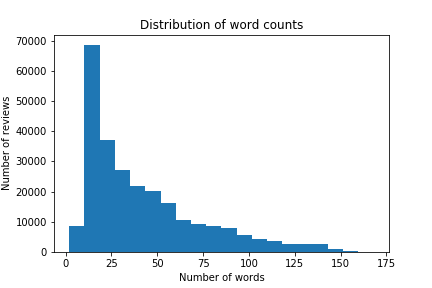
\includegraphics[scale=0.5]{wordcounts}
			\caption[scale=0.75]{Distribution of the word counts across the Glassdoor reviews.}
		\end{center}
	\end{figure}
	
	\begin{figure}[h]
		\begin{center}
			
\includegraphics[scale=0.75]{wordcloud}
			\caption[scale=0.75]{Word cloud of the reviews.}
		\end{center}
	\end{figure}
	
	\begin{table}[h]
		\begin{center}
			\begin{tabular}{|l|l|}
				\hline \textbf{Statistic} & \textbf{Value} \\ \hline
				Num of Observations & 259,317 \\
				Vocab Size & 110,897 \\
				Avg Review Length & 41 \\
				Max Review Length & 168 \\
				Min Review Length & 2 \\
				Avg Helpful Review Length & 57 \\
				Avg Not Helpful Review Length & 35 \\
				Pct Unhelpful Reviews & 71.24\% \\
				Pct Helpful Reviews & 28.76\% \\
				\hline
			\end{tabular}
			\caption[scale=0.75]{Descriptive Statistics on the Dataset.}
		\end{center}
	\end{table}
	
	
	\begin{table}[h]
		\begin{center}
			\begin{tabular}{|p{3cm}|p{5cm}|}
				\hline \textbf{Label} & \textbf{Review} \\ \hline
				Helpful & not too many benefits are about it. isolation - people are under a lot of pressure and it has been a bullying type of environment \\
				\hline
				Not Helpful & good people, good times, good atmosphere. hard to have any meaningful impact at any scale \\
				\hline
				Helpful & great salary \& stock options, decent food and other perks.. constantly reorging, lot's of pressure for promotion, sweatshop for designers, terrible commute if you don't live in mountain view. \\
				\hline
				Not Helpful & flexible working environment, great people, great perks, tons of opportunities across all types of disciplines... hard to get bored.. experience (positive or negative) can vary by manager \\
				\hline
			\end{tabular}
			\caption[scale=0.75]{Example Reviews}
		\end{center}
	\end{table}
	
	\subsection{Baseline SVM Model}
	Wang and Manning \cite{Wang} investigate two common baseline models for text classification: Multinomial Naive Bayes (MNB) and a linear Support Vector Machine (SVM). They train and test these models over four different datasets with varying input lengths, and find that MNB perform better at classifying snippets and short sentences, while SVMs outperforms at classifying longer strings of text like movie reviews. They also find that using bigrams word counts in sentence classification improves classification accuracy over unigrams, but using up to trigrams decreases accuracy. Based on these results, I decided to use a linear SVM and bigram counts for my baseline model. I chose the SVM over MNB because job reviews tend to be longer than just snippets, with an average review length of 41 words. Observations were divided into train and test datasets, which were used to train and evaluate the model. The baseline model achieves an accuracy score on the test set of \textbf{78.76\%}. Table 3 shows the normalized confusion matrix for the baseline model (H/NH indicates Helpful/Not Helpful):
	
	\begin{table}
		\begin{center}
			\begin{tabular}{lrr}
				\hline
				{} &  pred:NH &  pred:H \\
				\hline
				true:NH     &         0.664 &             0.046 \\
				true:H      &         0.167 &             0.123 \\
				\hline
			\end{tabular}
			\caption{Normalized Confusion Matrix for SVM}
		\end{center}
	\end{table}
	
	\subsection{CNN Model}
	CNNs have demonstrated exceptional results in text classification tasks. Kim \cite{Kim} showed that CNN variations improved on the state-of-the-art in 4 out of 7 sentence classification tasks, and still achieved excellent results compared to other neural network models and classical models with hand-coded features. Kim's model architecture consisted of:
	
	\begin{enumerate}
		\item An embedding layer, with one k-dimensional vector for each word
		\item A single 1-dimensional convolutional layer with multiple channels for different filter sizes
		\item A max-over-time pooling layer
		\item A fully-connected softmax layer that produces the predicted probabilities among the labels
	\end{enumerate}
	
	Kim's experiments included model variants where the embedding layer used word embeddings pre-trained by Mikolov et al.'s \cite{word2vec} Word2Vec algorithm, and showed that these pre-trained embeddings  consistently boosted classification performance compared to randomly initialized embeddings that are tuned as part of training. Zhang and Wallace \cite{Zhang} also find that using pre-trained word vectors enhances classification performance, and show that using either Word2Vec or GloVe \cite{Pennington} embeddings results in similar performance boosts. They do show, however, that allowing the embedding layer to be tuned during training uniformly outperforms CNN variants whether the embedding layer is held static. They also postulate that learning embeddings from scratch may have better results in datasets with many observations. Since my dataset is fairly large, I experimented with both using pre-trained GloVe embeddings in the embedding layer, and randomly initialized embeddings trained from scratch.
	
	Kim \cite{Kim} experiments with many different filter sizes and numbers of filters in the convolutional layer, but Zhang \cite{Zhang} suggests that optimal filter sizes for datasets with longer text is likely greater than 10. Their example was the Amazon Customer Reviews dataset from Hu and Liu \cite{Hu} (denoted as the ``CR" dataset in \cite{Zhang}), which has a max review length of 105. Since the max review length in my dataset is 165 words, I experiment with filter sizes up to 30. Zhang \cite{Zhang} also states that different numbers of filters can result in better performance, irrespective of the sentence length. I experiment with feature map sizes ranging from 10 to 400.
	
	Zhang and Wallace \cite{Zhang} experimented with different pooling strategies, and found that 1-max pooling consistently outperforms alternative pooling strategies like k-max pooling and average pooling. Additionally, they experiment with different dropout rates after the pooling layer to regularize their CNN models, and find that varying the dropout rate does not materially affect performance, except for dropout rates above 0.7, which almost uniformly perform poorly. I used 1-max pooling in my experiments, but did experiment with different dropout rates.
	
	\section{Results}
	I began with an initial set of architecture and hyperparameter configurations:
	\begin{itemize}
		\item Filter sizes of 5, 15, and 30
		\item 100 filters per size
		\item Randomly-initialized embeddings
	\end{itemize}
	
	I experimented with different dropout rates, then different numbers of filters, and then using pre-trained embeddings.
	
	\subsection{Dropout Rate}
	Contrary to the results observed in Kim \cite{Kim} and Zhang \& Wallace \cite{Zhang}, I observed that tuning the dropout rate in the penultimate layer had a significant impact on the results. I iterated over 10 different dropout rates from 0.0 to 0.9 in increments of 0.1, and found that test set accuracy almost monotonically increased as the dropout rate increase, with the lowest accuracy being 69.86\% and highest being 74.53\%. Figure 3 illustrates 
	
	\begin{figure}[h]
		\begin{center}
			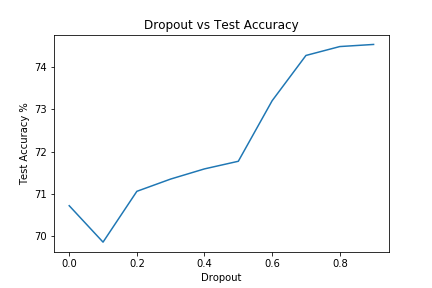
\includegraphics[scale=0.5]{dropout}
			\caption[scale=0.75]{Accuracy Score vs Dropout Rate}
		\end{center}
	\end{figure}
	
	
	\subsection{Number of Filters}
	I experimented with different numbers of filters: 10, 25, 50, 100, 200, 400. I found that the number of filters had little effect on model performance. Accuracy scores ranged from 74.29\% to 74.82\%, and did not correlate with the number of filters. This doesn't diverge much from the results that Zhang and Wallace \cite{Zhang}, where they observed that increasing the number of filters boosted performance, but only slightly.
	
	
	\subsection{Filter Sizes}
	I also experimented with models that have a single filter sizes, but different values for the filter sizes - 1, 3, 5, 7, 11, and 15. I held the numbers of filters the same at 100. Table 4 shows the results:
	\begin{table}[h]
		\begin{center}
			\begin{tabular}{|l|l|}
				\hline \textbf{Filter Size} & \textbf{Accuracy Score} \\ \hline
				1 & 74.02\% \\
				3 & 74.34\% \\
				5 & 73.84\% \\
				7 & \textbf{74.41\%} \\
				11 & 74.22\% \\
				15 & 74.12\% \\
				\hline
			\end{tabular}
			\caption[scale=0.75]{Filter sizes and accuracy scores.}
		\end{center}
	\end{table}
	
	Adjusting the filter size seemed to make little difference in boosting performance in this classification task.
	
	
	\subsection{Pre-trained vs Untrained Embeddings}
	I found that using pre-trained embeddings at the start of training resulted in an increase in accuracy score. With the default settings and a Dropout rate of 0.9, initializing the embedding matrix to use pre-trained GloVe embeddings resulted in an accuracy score of 75.35\%, which is a 0.82\% improvement over the untrained embeddings. This differed from the results that Kim \cite{Kim} and Zhang \& Wallace \cite{Zhang}, who both observed significant performance boosts from incorporating pre-trained embeddings in their models. This difference is likely due the size of the Glassdoor dataset being much larger, thus giving the randomly-initialized embeddings enough data to learn better-fitting dense representations of the words. 
	
	
	\subsection{Dataset Noisiness and Overfitting}
	Throughout the experimentation, I experienced overfitting in models with low dropout rates, with the training set accuracy score finishing above 98\% in the last epoch but the validation set accuracy score consistently declining as the epochs progressed before settling below 70\% at the end of the last epoch. Figure 4 illustrates this overfitting in the initial configuration with a dropout rate of 0.2.
	
	\begin{figure}[h]
	\begin{center}
		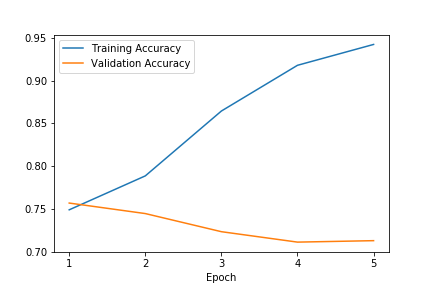
\includegraphics[scale=0.5]{overfitting}
		\caption[scale=0.75]{Train/Validation Accuracy Score at each Epoch with Dropout Rate of 0.2}
	\end{center}
	\end{figure}

	I suspect this was due to the noisiness in the dataset's labels. The data collected was a point-in-time snapshot of what was on the website, which included reviews that would likely be indicated as Helpful, but users had not yet voted it because they were freshly posted. Likewise, many reviews that were posted years ago and voted as Helpful did not appear to be more useful than reviews not voted as helpful. Table 5 lists a few examples of these false positives and negatives.
	
	\begin{table}[h]
	\begin{center}
	\begin{tabular}{|p{1.7cm}|p{5cm}|}
	\hline \textbf{Label} & \textbf{Text} \\ \hline
	``Helpful" & great company with great benefits. you are a number \\
	\hline
	``Helpful" & work culture, work / life balance. great company with competitive pay \\
	\hline
	``Unhelpful" & flexible hours, decent pay, helpful bosses, fun perks. although tech aide positions aren't the greatest thing in the world, they are very good for...\\
	\hline
	``Unhelpful" & very good 401k match. 6\% dollar for dollar. not much else is worth mentioning.. too many meetings. corporate pours millions into the headquarters while squeezing the remote sites...\\
	\hline
	\end{tabular}
	\caption[scale=0.75]{Examples of Likely False Positives and Negatives.}
	\end{center}
	\end{table}
	
	This is likely why the simpler baseline model outperformed all of the CNN models, and why models higher dropout rates tended to result in better performance.

	\section{Conclusion}
	In this paper I experimented with using CNNs to classify the helpfulness of job reviews. The dataset I built was noisy, and led to the neural network models to overfit without a high dropout rate, and resulted in the more complex CNN models to underperform the baseline SVM model. I performed a sensitivity analysis of the model configurations on the accuracy score. Because of the dataset's noisiness compared to more canonical sentence classification datasets, I observed some results that differed from similar previous literature: tuning the dropout rate significantly boosted performance, but tuning the filter sizes and number of filters did not impact performance at all. Pre-trained embeddings increased accuracy score, though not as significantly as in previous papers. This adds to the literate on text classification with Convolutional Neural Networks with noisy datasets.
	
	
	\bibliographystyle{plain}
	\bibliography{glassdoor}
	
	
	
\end{document}
